\chapter{АНАЛИЗ ТЕКУЩИХ РЕШЕНИЙ ПОЛУЧЕНИЯ, АНАЛИЗА И ОБРАБОТКИ ЭКСПЕРТНОЙ ИНФОРМАЦИИ В ОБЛАСТИ ОБСЛУЖИВАНИЯ ПРОГРАММНОГО ОБЕСПЕЧЕНИЯ И ИНФОРМАЦИОННОЙ ИНФРАСТРУКТУРЫ} \label{chapt3}

\section{Обзор решений} \label{sect3_1}

\textbf{HP OpenView} \cite{HPOpenView} является комплексным программным решением по мониторингу ИТ инфраструктуры предприятия. Система имеет множество модулей. Данная система охватывает широкий спектр возможностей:
\begin{itemize}
	\item Мониторинг
	\item Регистрация инцидентов
	\item Управление системами
\end{itemize}
Система не поддерживает:
\begin{itemize}
	\item Понимание и формализация запросов
	\item Автоматическое исправление проблемы на основе формализации запроса
\end{itemize}


\begin{figure} [h] 
  \center
  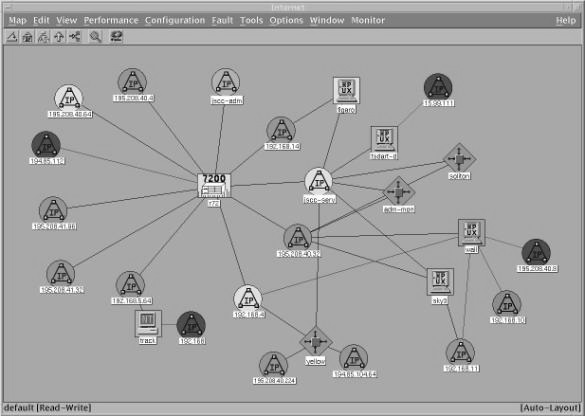
\includegraphics [scale=1.0] {hpopenview}
  \caption{HP OpenView} 
  \label{img:hpopenview}  
\end{figure}

\textbf{ServiceNOW} Средства автоматизации сервиса. Предоставляет следующие возможности:
\begin{itemize}
	\item Регистрация инцидентов
	\item Создание цепи обработки инцидента
\end{itemize}

Система не поддерживает:
\begin{itemize}
	\item Понимание и формализация запросов
	\item Автоматическое исправление проблемы на основе формализации запроса
\end{itemize}


\begin{figure} [h] 
  \center
  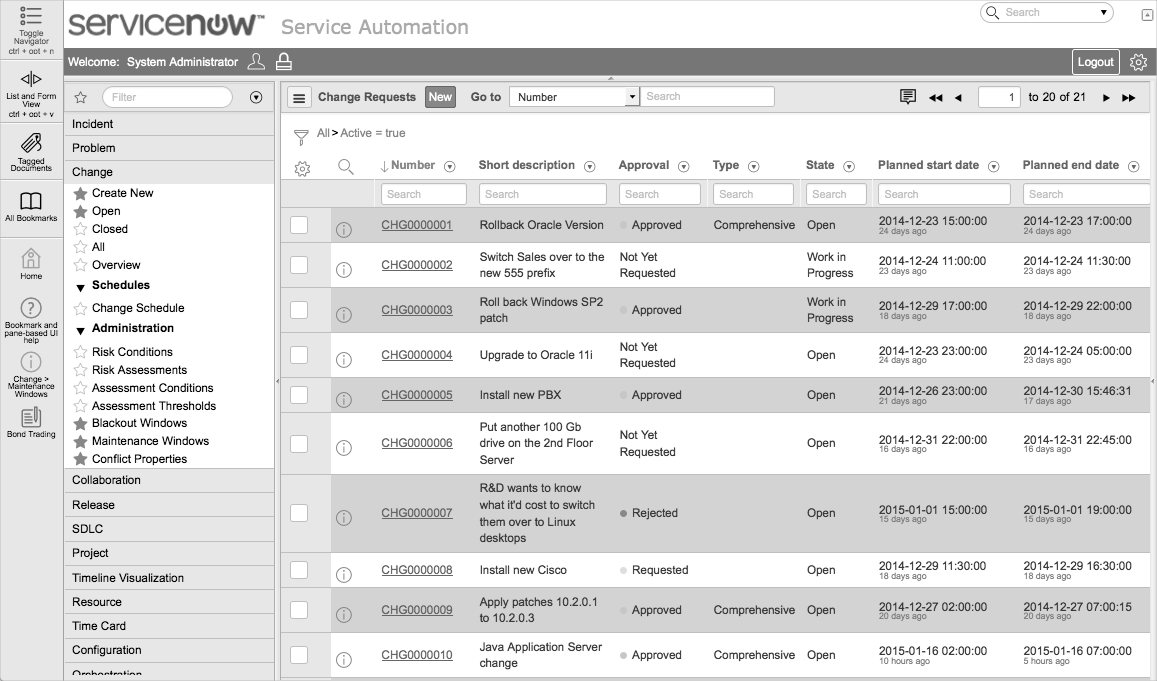
\includegraphics [scale=0.3] {svnow}
  \caption{Service NOW} 
  \label{img:svnow}  
\end{figure}

\textbf{Прочие системы}
Кроме того существуют дополнительные способы автоматизации
\begin{itemize}
	\item Обработка инцидентов посредством регулярных выражений. В таком решение нет гибкости, так как обработка идет путем поиска ключевых слов вне контекста
	\item Обработка инцидентов при помощи скриптов. Автоматизирует лишь рутинные операции
\end{itemize}

\clearpage
\section{Требования к системе} \label{sect3_2}

Основными требованиями к системе является следующие:
\begin{itemize}
	\item Понимание входящий информации на естественном языке
	\item Формализация инцидента в контексте
	\item Поиск решение инцидента
	\item Обучение решению инцидента
	\item Умение проводить логические рассуждения: генерализацию, специализацию, синонимичный поиск
	\item Умение мыслить
\end{itemize}

Требования к системе формировались исходя из возможностей специалистов поддержки, а также анализа проблем, которыми они занимаются. Большинство инцидентов тривиальные и типичные, но все они разные. Для человека проблема "Please insall Firefox" и "Please install Chrome" идентичные, но с точки зрения формализации - нет. Общее в них можно найти взглянув на генерализацию различающейся части. Firefox и Chrome являются пакетами программного обеспечения.




\clearpage